\subsection{Stopped Proton}

Protons are selected by the information of beam counters.
Proton events are applied following simple selections.
The drift time of the hit at the injection point are restricted from 150$mu$s to 300$\mu$s which corresponds with BDC fiducial volume.
The total hit number in the cluster is greater than 5.
Only one hit are required at the same channel in the cluster to remove multi-track events.
Then, we define the events which the number of clusters in the event which passed above selections is only one as good proton events.
For good proton events, we compare each parameter between data and MC.
Figure\ref{fig:various_distribution} shows the comparison of the distribution of Hit Charge, Hit Sigma, Stopped Channel and  Cluster Charge between data and MC.
All four distributions of MC reproduce data well.
Especially, the agreement of stopped channel distribution shows the consistent the momentum estimation by TOF information with the initial momentum of the particles injected to 250L detector.\\

\begin{figure}[htbp]
  \centering
  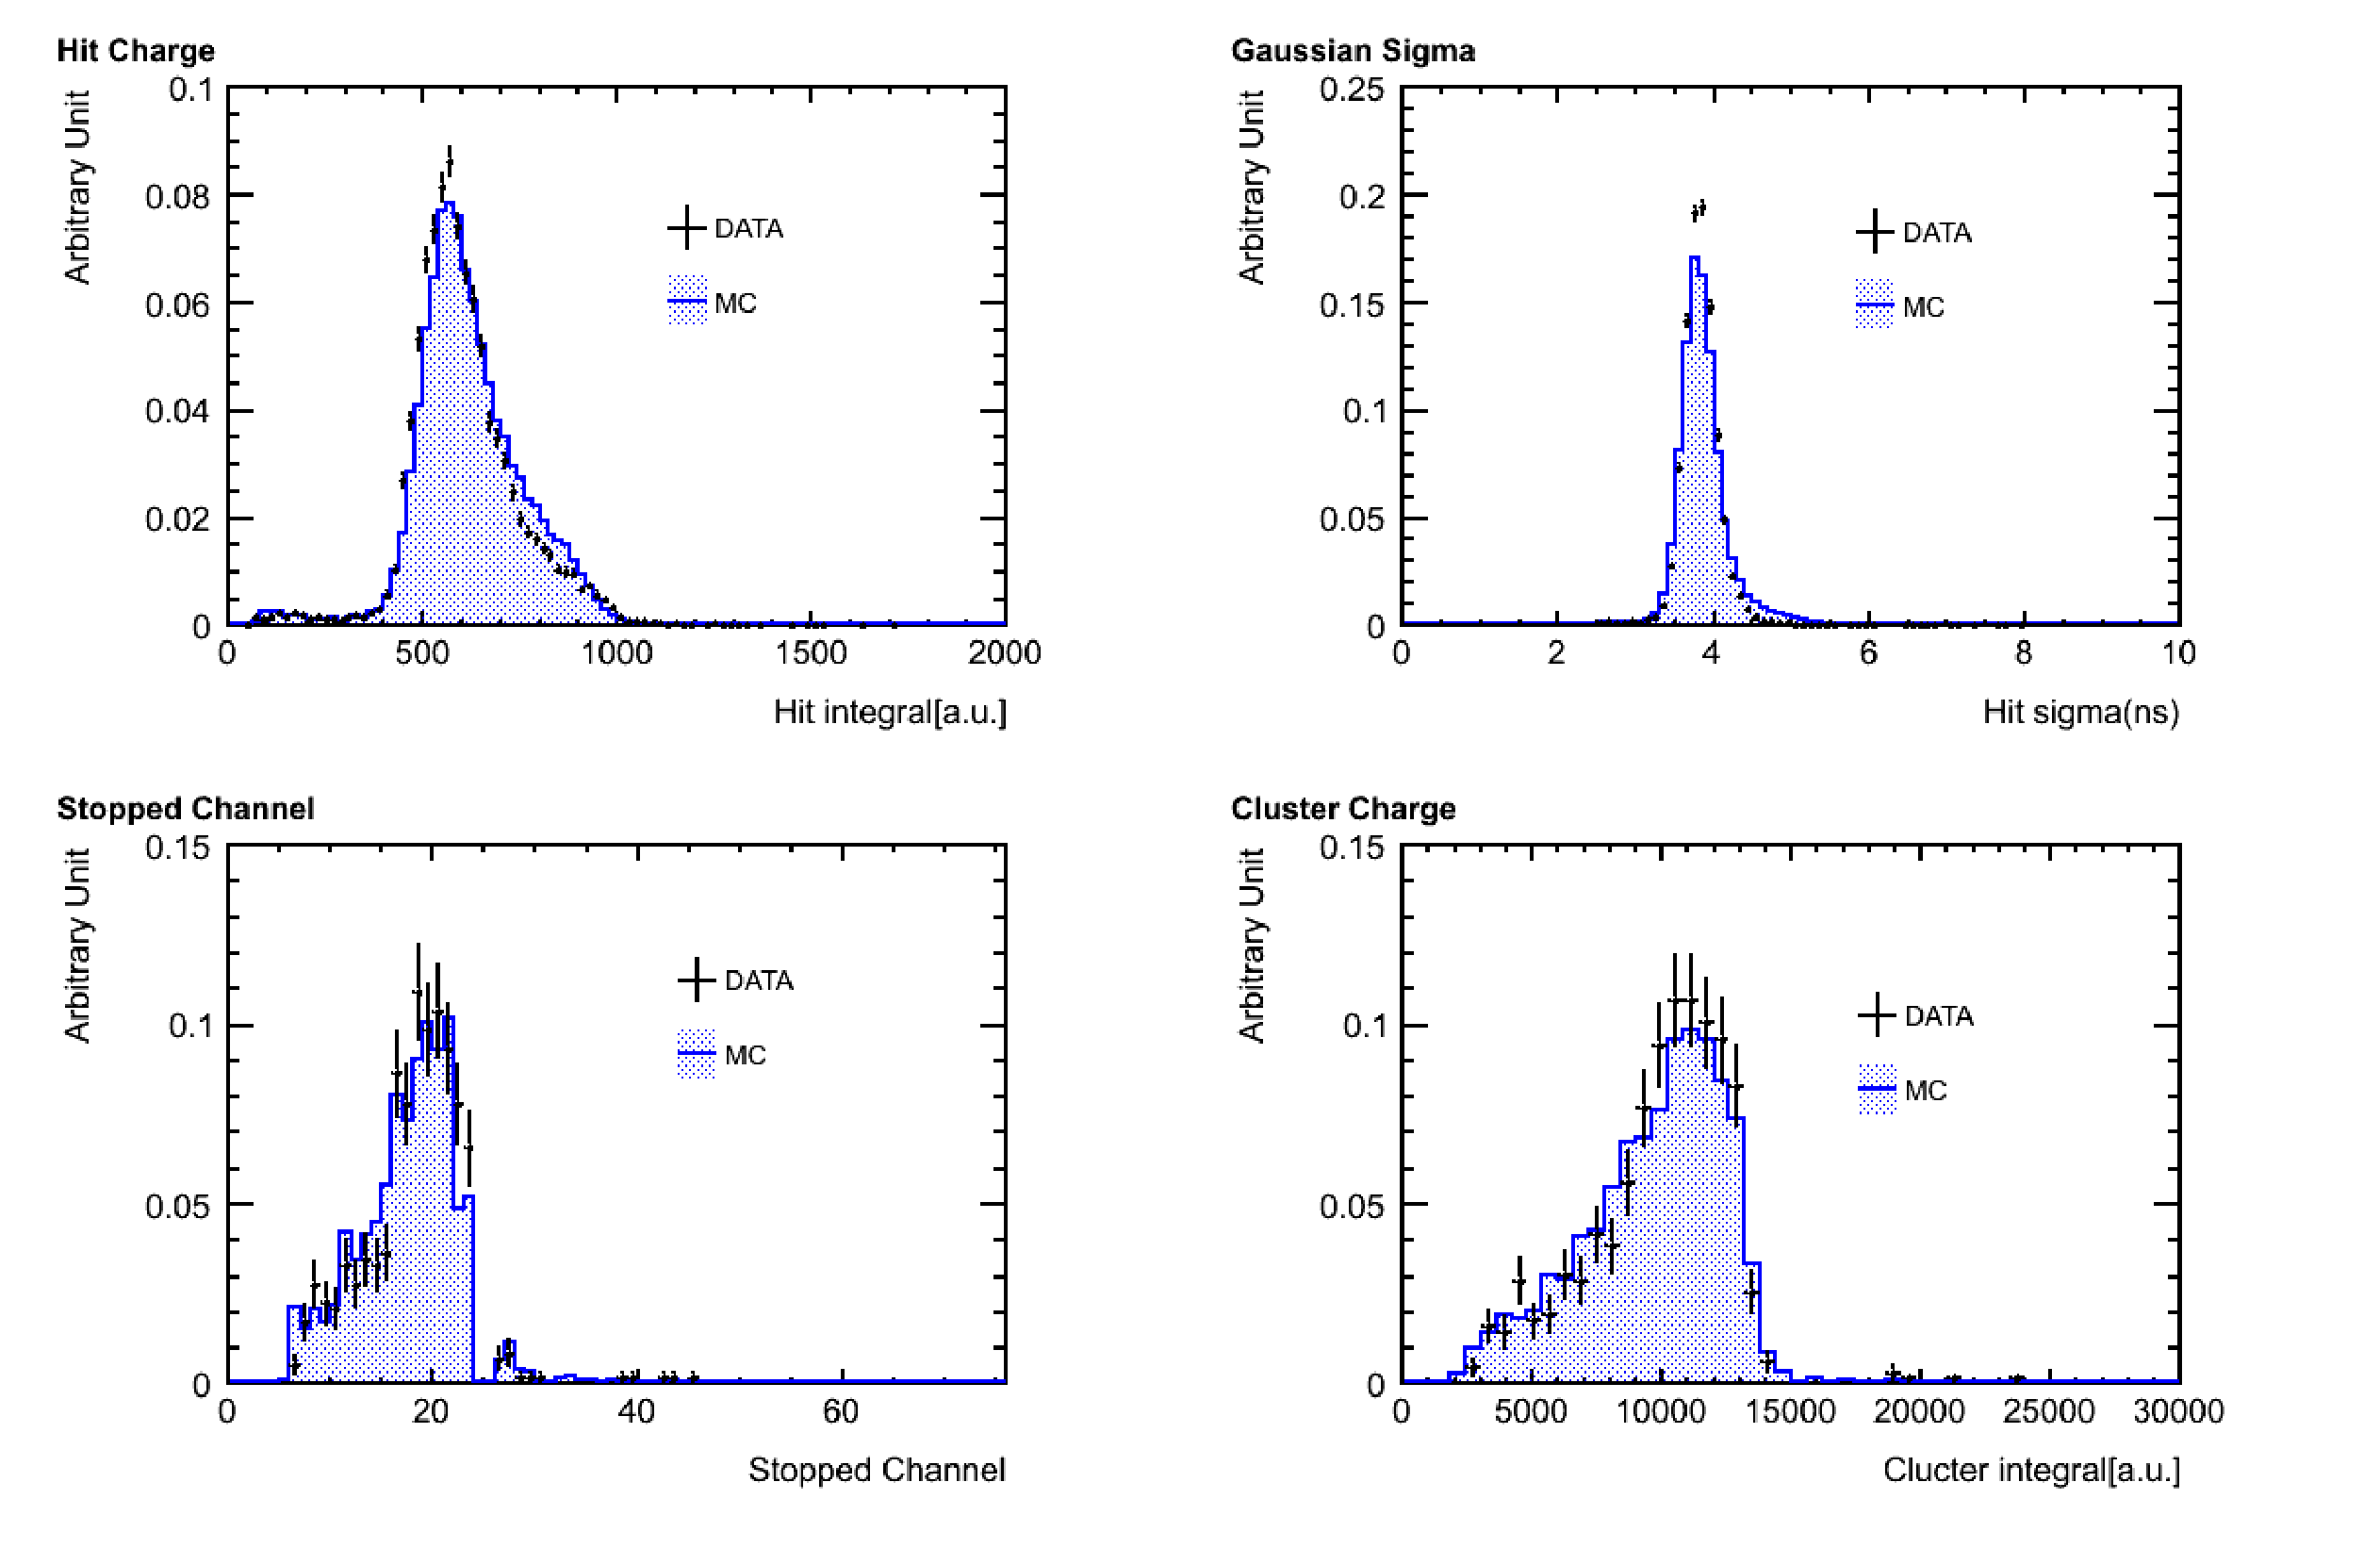
\includegraphics[width=10cm,clip]{./fig/stop_proton1.eps}
  \caption{Hit Charge, Hit Sigma, Stopped Channel, Cluster Charge}
  \label{fig:varios_distribution}
\end{figure}

Figure\ref{fig:ADC_distribution} shows the hit charge distribution of each distance from stopped point.
Hit charge distributions of MC simulation are good agreements with data.\\
Figure\ref{fig:Mean_comparison} shows the mean of the above distribution of each distance.
Figure\ref{fig:Mean_comparison_ratio} shows the ratios of Data/MC.
The ratios are within 94\%$\sim$105\%.
From this result, MC simulation reproduce the charge response of data in high and wide dE/dx region well.

\begin{figure}[htbp]
  \centering
  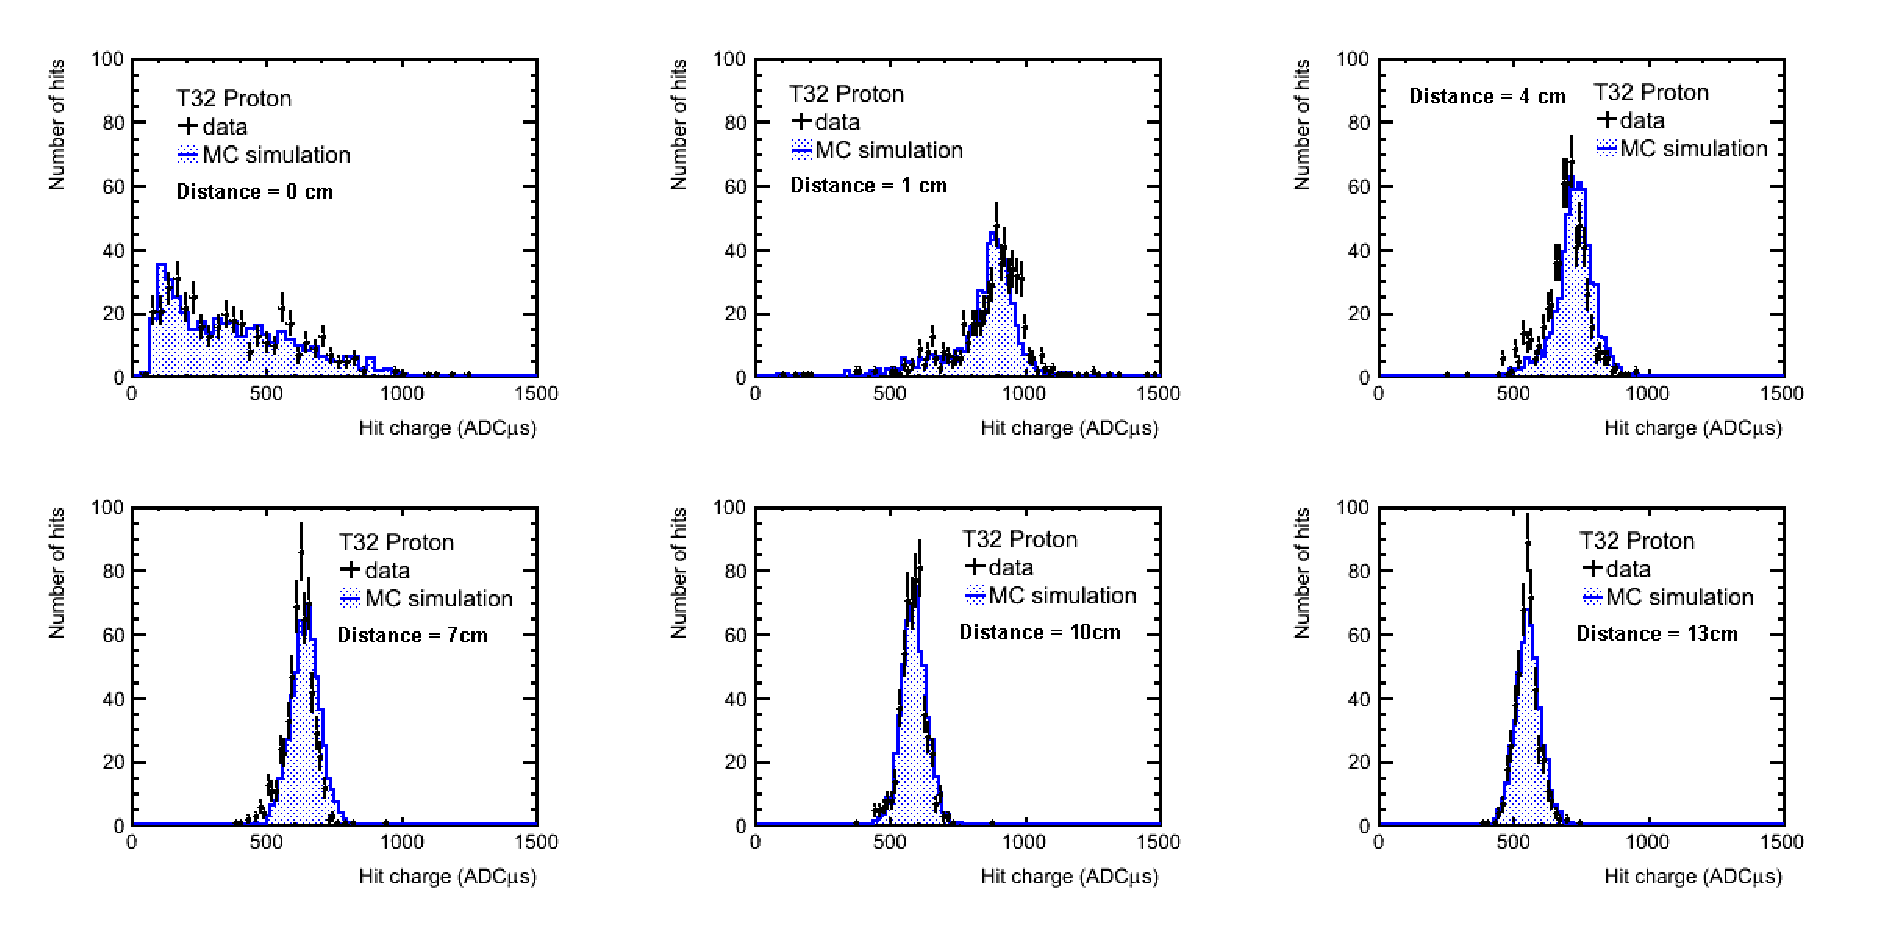
\includegraphics[width=10cm,clip]{fig/stop_proton2.eps}
  \caption{Hit charge distribution of each distance from stopped point}
  \label{fig:ADC_distribution}
\end{figure}

\begin{figure}[htbp]
  \begin{tabular}{cc}
    \begin{minipage}{0.5\hsize}
      \centering
      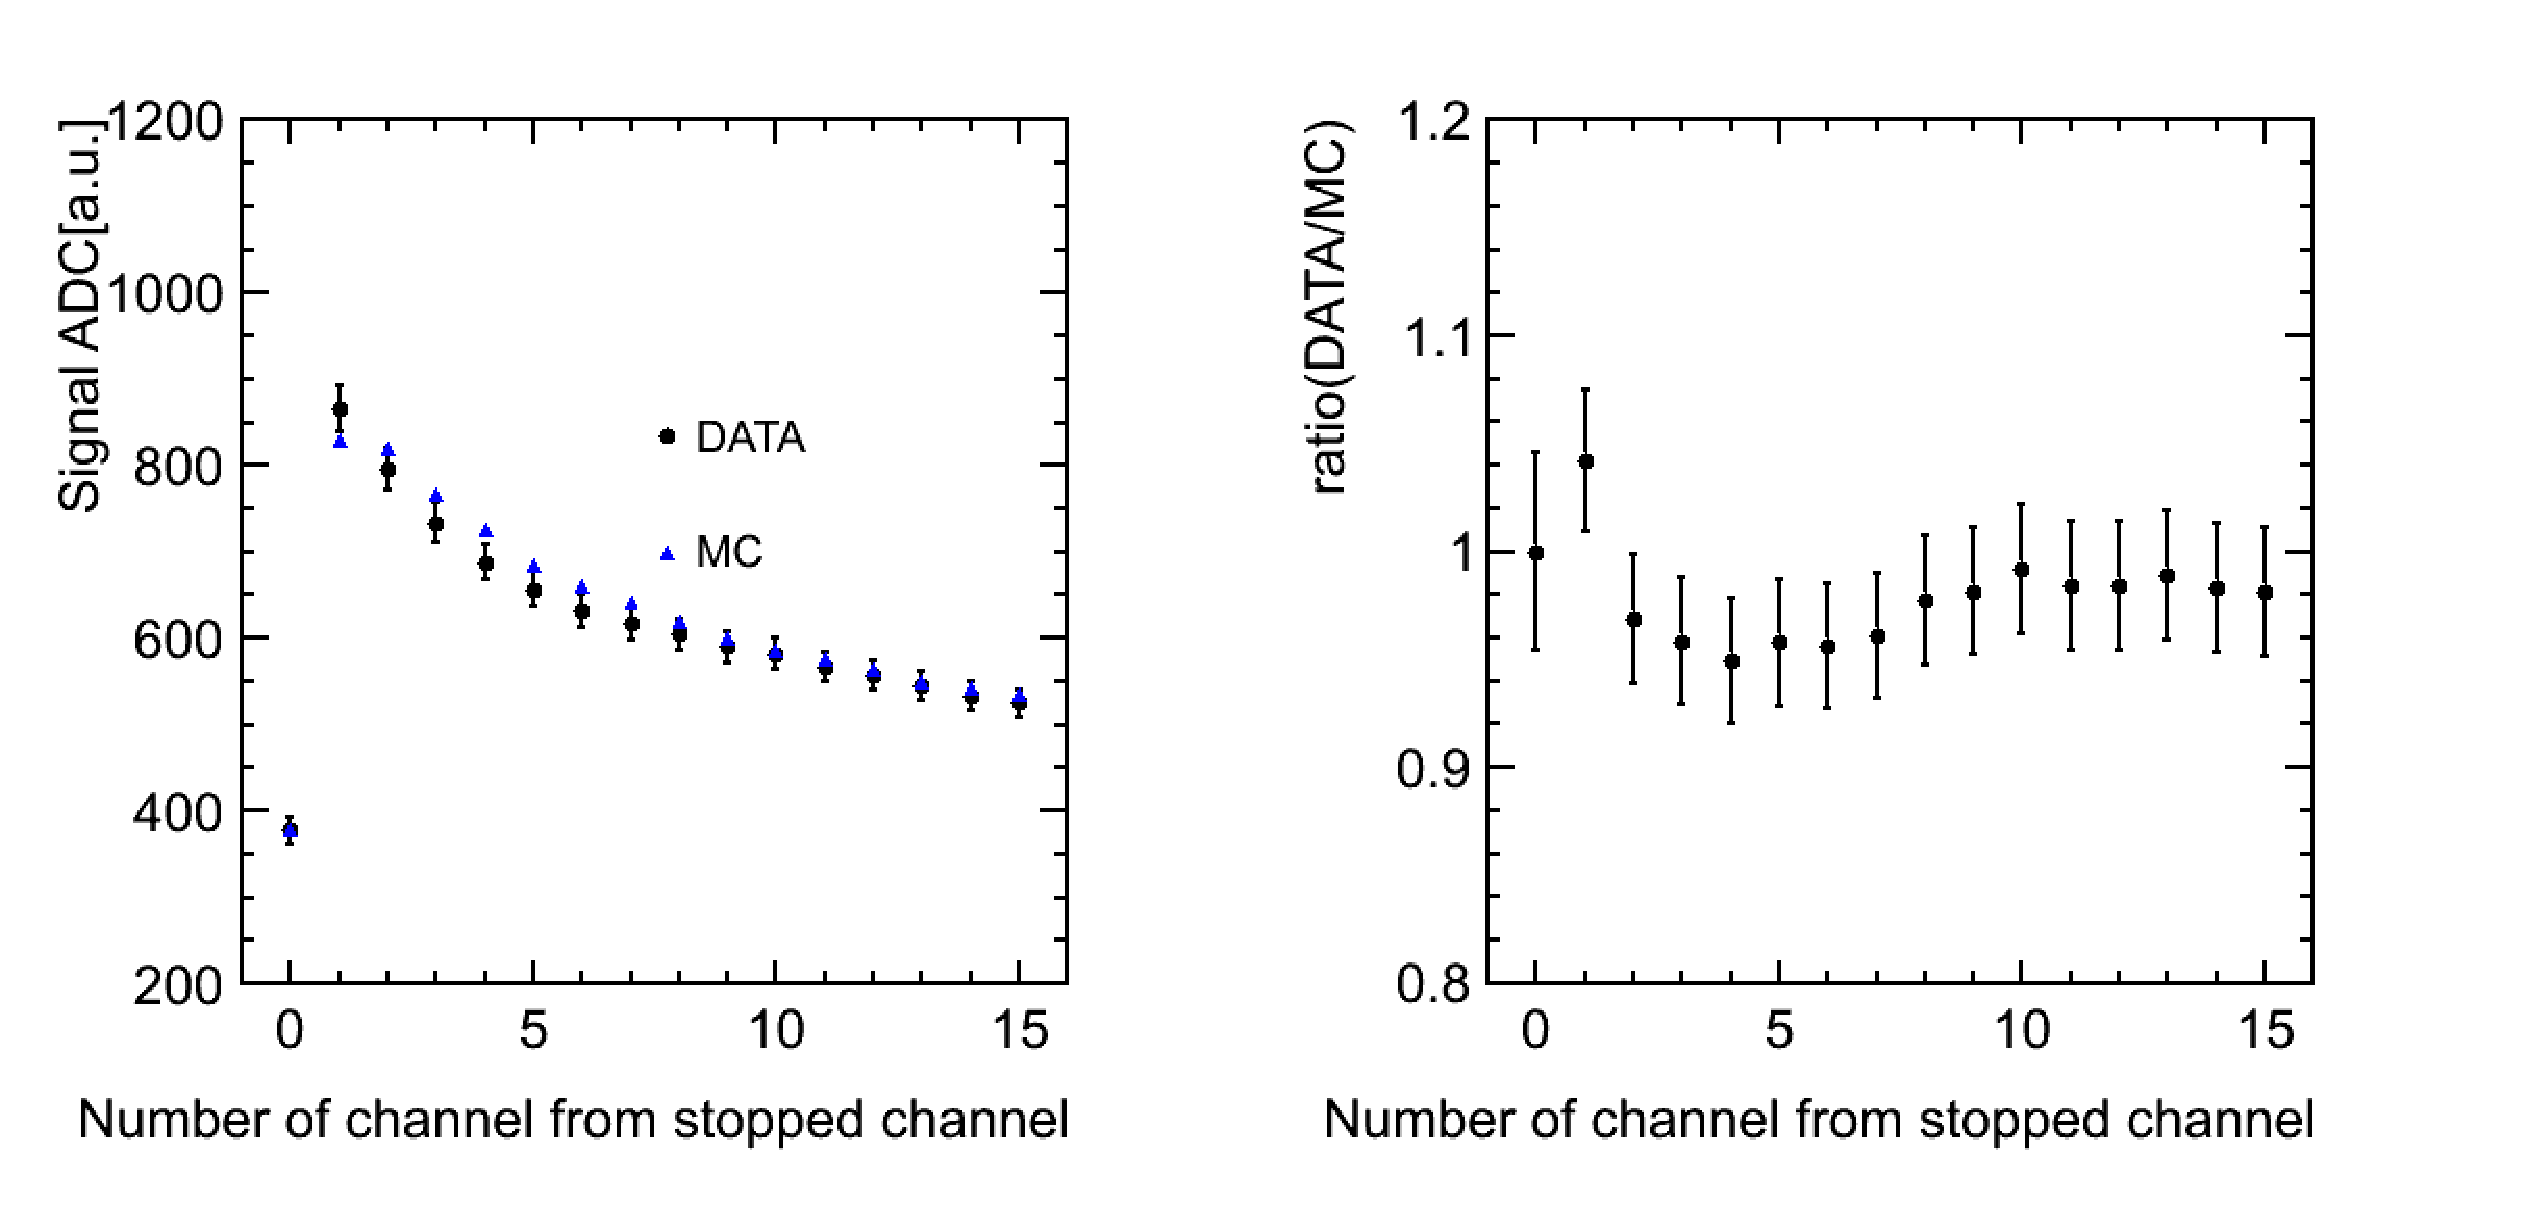
\includegraphics[width=6cm,clip]{fig/stop_proton3.eps}
      \caption{Data-MC comparison of the mean of hit charge distribution}
      \label{fig:Mean_comparison}
    \end{minipage}
    \begin{minipage}{0.5\hsize}
      \centering
      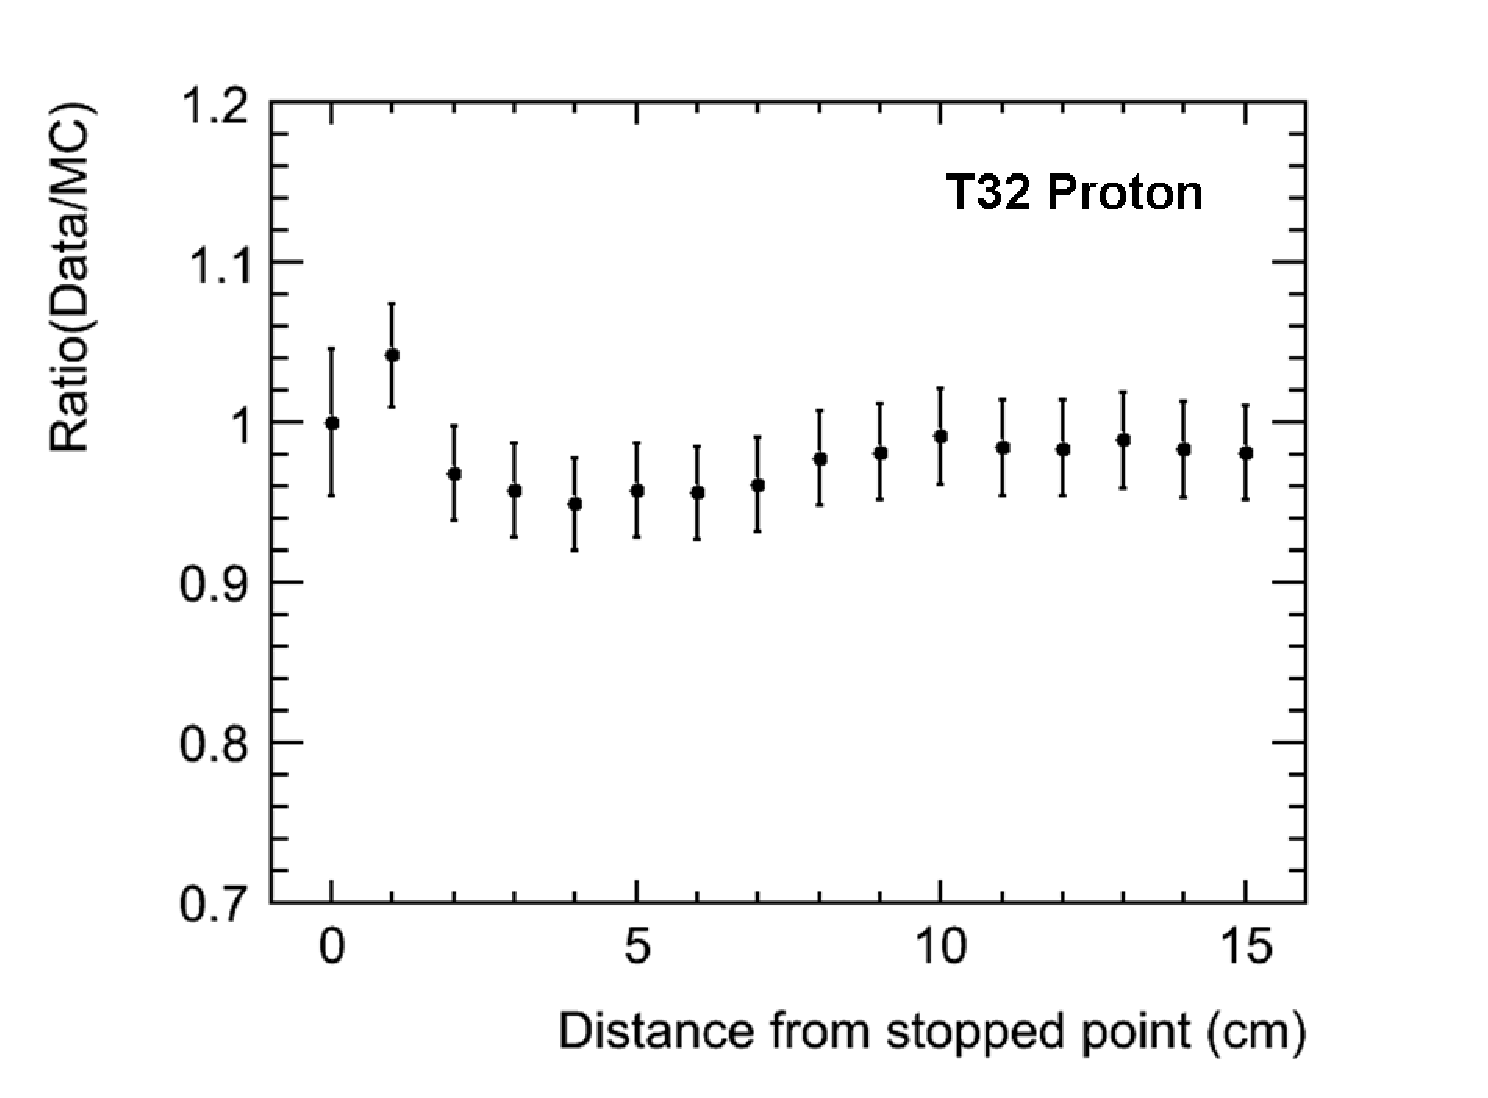
\includegraphics[width=6cm,clip]{fig/stop_proton4.eps}
      \caption{Data-MC comparison of the ratio of the mean}
      \label{fig:Mean_comparison_ratio}
    \end{minipage}
  \end{tabular}
\end{figure}

% LocalWords:  fiducial
